%%%%%%%%%%%%%%%%%%%%%%%%%%%%%%%%%%%%%%%% IMPORTS %%%%%%%%%%%%%%%%%%%%%%%%%%%%%%%%%%%%%%%%
\documentclass[11pt,onesize,a4paper,titlepage]{article}

%%%%%%%%%%%%%%% Formatting %%%%%%%%%%%%%%% 
\usepackage[english]{babel}
\usepackage[utf8]{inputenc}
\usepackage{geometry} % Margins
\usepackage{sectsty} % Custom Sections

%%%%%%%%%%%%%%% Font %%%%%%%%%%%%%%% 
\usepackage{Archivo}
\usepackage[T1]{fontenc}

%%%%%%%%%%%%%%% Graphics %%%%%%%%%%%%%%% 
\usepackage{fontawesome5} % Icons
\usepackage{graphicx} % Images
\usepackage[most]{tcolorbox} % Color Box
\usepackage{xcolor} % Colors
\usepackage{tikz} % For Drawing Shapes
\tcbuselibrary{breakable}

%%%%%%%%%%%%%%% Miscelanous %%%%%%%%%%%%%%% 
\usepackage{lipsum} % Lorem Ipsum
\usepackage{hyperref} % For Hyperlinks

%%%%%%%%%%%%%%% Colors %%%%%%%%%%%%%%% 
\definecolor{title}{HTML}{4bfbba} % Color of the title
\definecolor{backdrop}{HTML}{f2f2f2} % Color of the side column
\definecolor{lightgray}{HTML}{b8b8b8} % Color for the skill bars

%%%%%%%%%%%%%%% Section Format %%%%%%%%%%%%%%% 
\sectionfont{                     
    \LARGE % Font size
    \sectionrule{0pt}{0pt}{-8pt}{1pt} % Rule under Section name
}

\subsectionfont{
    \large % Font size
    \fontfamily{phv}\selectfont % Font family
    \sectionrule{0pt}{0pt}{-8pt}{1pt} % Rule under Subsection name
}

%%%%%%%%%%%%%%% Margins and Headers %%%%%%%%%%%%%%%
\geometry{
  a4paper,
  left=7mm,
  right=7mm,
  bottom=10mm,
  top=10mm
}

\pagestyle{empty} % Empty Headers
%%%%%%%%%%%%%%%%%%%%%%%%%%%%%%%%%%%%%%%% MACROS %%%%%%%%%%%%%%%%%%%%%%%%%%%%%%%%%%%%%%%%

%%%%%%%%%%%%%%% Link With an Icon %%%%%%%%%%%%%%% 
\newcommand{\link}[1]{
    \href{#1}{\faIcon{link}}
}

%%%%%%%%%%%%%%% Name Template %%%%%%%%%%%%%%% 
\newcommand{\name}[2]{
    % Name
    \Huge % Font size
    \raggedright \textbf{#1} \par

    \vspace*{0.3cm}
    
    % Profession
    \Large % Font size
    \raggedright #2 \par
    \normalsize \normalfont
}

%%%%%%%%%%%%%%% Contact Details %%%%%%%%%%%%%%%
\newcommand{\info}[2]{
    \faIcon{#2} \hspace{0.2em} #1
}

%%%%%%%%%%%%%%% Email %%%%%%%%%%%%%%%
\newcommand{\email}[1]{
    \info{#1}{envelope}
}

%%%%%%%%%%%%%%% Phone Number %%%%%%%%%%%%%%%
\newcommand{\phone}[1]{
    \info{#1}{mobile-alt}
}

%%%%%%%%%%%%%%% Address %%%%%%%%%%%%%%%
\newcommand{\address}[1]{
    \info{#1}{map-marker-alt}
}

%%%%%%%%%%%%%%% GitHub %%%%%%%%%%%%%%%
\newcommand{\github}[2]{
    \info{\href{#1}{\underline{#2}}}{github}
}

%%%%%%%%%%%%%%% LinkedIn %%%%%%%%%%%%%%%
\newcommand{\linkedin}[2]{
    \info{\href{#1}{\underline{#2}}}{linkedin}
}

%%%%%%%%%%%%%%% Website %%%%%%%%%%%%%%%
\newcommand{\website}[1]{
    \info{#1}{link}
}

%%%%%%%%%%%%%%% Draw Skill Bars %%%%%%%%%%%%%%% 
\newcommand{\drawskillbars}[1]{
    \begin{tikzpicture}
        % Draw 5 gray bars
        \foreach \i in {0, 1, 2, 3, 4}{
            \fill[lightgray] (\i * 0.7 + 0.2 *\i,0) rectangle (0.7 + \i * 0.7 + \i * 0.2,0.1);
        }
        
        % Draw number of black bars depending on the skill level
        \foreach \i in {#1}{
            \fill[black] (\i * 0.7 + 0.2 *\i,0) rectangle (0.7 + \i * 0.7 + \i * 0.2,0.1);
        }
    \end{tikzpicture} \par
}
    
%%%%%%%%%%%%%%% Skills %%%%%%%%%%%%%%%
\newcommand{\skill}[2]{
    % Name of the skill
    \large
    \noindent \hangafter=0
    \textmd{#1}
    \normalsize \par 
    % Skill bars
    \drawskillbars{#2}
    \vspace{1.5em}
}

\newcommand{\cvtag}[1]{%
    \tikz[baseline]\node[anchor=base,draw=body!30,rounded corners,inner xsep=1ex,inner ysep =0.75ex,text height=1.5ex,text depth=.25ex]{#1};
}

%%%%%%%%%%%%%%% Language %%%%%%%%%%%%%%%
\newcommand{\lan}[2]{
    % Name of the language
    \large
    \noindent \hangafter=0
    \textmd{#1}
    % Knowledge level
    \drawskillbars{#2}
    \vspace{1em}
 }

%%%%%%%%%%%%%%% Education %%%%%%%%%%%%%%%
\newcommand{\education}[4]{
    % Name of the studies
    \noindent \large \parbox{.7\linewidth}{\textbf{#1}}
    % Duration in a Box
    \hfill \scriptsize
    \tcbox[enhanced,box align=base,nobeforeafter,colback=title,colframe=title,size=fbox,arc=0mm]{\textbf{#2}} \par
    \vspace{0.3em}
    % School Name 
    \large
    \noindent \color{emphasis} \parbox{.7\linewidth}{\textsl{#3}} \par
    % Description
    \normalsize \color{black}
    \vspace*{0.3em}
    \small #4 
    \normalsize \par
}

%%%%%%%%%%%%%%% Work Experience %%%%%%%%%%%%%%%
\newcommand{\work}[4]{
    % Name of the Job
    \noindent \large \parbox{.7\linewidth}{\textbf{#1}}
    % Duration in a Box 
    \hfill \scriptsize
    \tcbox[enhanced,box align=base,nobeforeafter,colback=title,colframe=title,size=fbox,arc=0mm]{\textbf{#2}} \par
    \vspace{0.3em}
    % Name of the Employer
    \noindent \large \color{emphasis} \parbox{.7\linewidth}{\textsl{#3}} \par
    % Description of the job
    \vspace*{0.3em} \color{black}
    \small #4 
    \normalsize \par
}

%%%%%%%%%%%%%%% Publications %%%%%%%%%%%%%%%
\newcommand{\pub}[5]{
    % Title
    \noindent \large \parbox{.7\linewidth}{\textbf{#1} \link{#5}}
    % Publication Date
    \hfill \scriptsize
    \tcbox[enhanced,box align=base,nobeforeafter,colback=title,colframe=title,size=fbox,arc=0mm]{\textbf{#2}} \par
    \vspace{0.3em}
    % Institution
    \large
    \noindent \color{title} \parbox{.7\linewidth}{\textsl{#3}} \par
    % Description
    \vspace*{0.3em} \color{black}
    \small \textit{#4} \par
    \normalsize \par 
}

\RequirePackage{accsupp}
\definecolor{PastelBlack}{HTML}{292929} % PastelRed 8F0D0D
\definecolor{SlateGrey}{HTML}{2E2E2E}
\colorlet{accent}{PastelBlack}
\colorlet{emphasis}{SlateGrey}

% defined for my use
\newcommand{\cvDateMarker}{\faCalendar[regular]}

\newcommand{\cvevent}[5]{%
  {\large\color{emphasis}\textbf{#1}\par} % Event title
  \smallskip\normalsize

  \ifstrequal{#3}{}{}{%
    {\small\makebox[0.5\linewidth][l]%
      {\BeginAccSupp{method=pdfstringdef,ActualText={\datename:}}\cvDateMarker\EndAccSupp{}%
      ~#3}%
    }}%
  \ifstrequal{#4}{}{}{%
    {\small\makebox[0.5\linewidth][l]%
      {\BeginAccSupp{method=pdfstringdef,ActualText={\locationname:}}\cvLocationMarker\EndAccSupp{}%
        ~#4}%
    }}\par \newline

  \ifstrequal{#2}{}{}{%
    \textbf{\color{accent}#2}\par
    \smallskip
  }
  \ifstrequal{#5}{}{}{%
    \small #5 \par
  }
  \medskip\normalsize
}


\begin{document}
        %%% TItle %%%
        \tcbset{colframe=title,colback=title,arc=0mm}
        \begin{tcolorbox}
    
            \begin{minipage}{0.3\textwidth} % Picture Area
                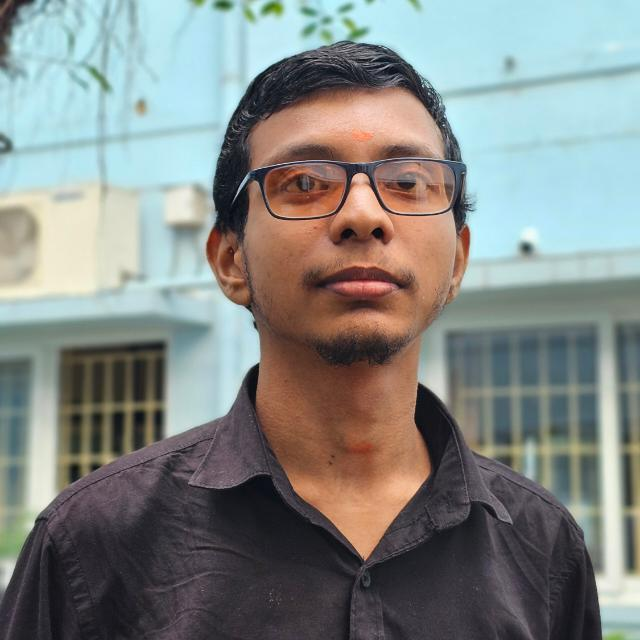
\includegraphics[width=0.8\textwidth]{profile.jpg} % Picture
            \end{minipage} \hfill
            \begin{minipage}{0.65\textwidth} % Name and Contact Info
               \name{Gowtham.S}{\small Tech Enthusiast | Passionate Developer from India | Aficionado of CLI, Linux, and Open-Source | Crafting Elegant Solutions with Precision ⚡️} % Name and Profession
                \vspace{1em}
                \email{gowtham.sri@zohomail.in} $\cdot$
                \phone{+91 739-58-31324} \par \vspace{0.5em}
                \address{Tamil Nadu, India} $\cdot$
                \github{https://github.com/silentFellow}{silentFellow} $\cdot$
                \linkedin{https://www.linkedin.com/in/silentFellow}{silentFellow} $\cdot$
                
                \newcommand{\webpage}[2]{\href{#1}{\faGlobe\ #2}}
                \webpage{https://gowtham-portfolio-5idn.onrender.com}{Portfolio}
            \end{minipage}
            
        \end{tcolorbox}

    %%% Sections %%%
    \vspace*{-1em}
    \tcbset{colframe=white,colback=white,arc=0mm, height=0.8\textheight}
    \begin{tcolorbox}
        \vspace*{-0.5em}
        \begin{minipage}[t]{0.3\textwidth} % Side Panel (e.g. Skills, Links, Languages, etc.)
            \begin{tcolorbox}[height=0.8\textheight, grow to left by=0.6cm,colback=backdrop,colframe=backdrop,arc=0mm]

                % Skills, the skill level is drawn as bars, input: skill name and an array starting from 0 and ending before 4
                \subsection*{Tech Stack}
                    \skill{Golang}{0, 1, 2, 3,4}
                    \skill{JavaScript/TypeScript \newline \textit \textit{(React, NextJs, NodeJs)}
}{0, 1, 2,3,4}
                    \skill{Python}{0, 1, 2, 3}
                    \skill{C, C++, Java}{0, 1, 2,}

                \subsection*{Tech Toolbox}
                    {\LaTeXraggedright
                        \cvtag{Linux (Advanced)}
                        \cvtag{Neovim}
                        \cvtag{Git}
                        \cvtag{Docker}
                        \cvtag{MongoDB}
                        \cvtag{PostgresSQL}
                        \cvtag{AWS}
                        \cvtag{Markdown}
                        \cvtag{Cred}
                        \cvtag{Ente-Auth}
                        \cvtag{Bruno}
                    \par}

                \subsection*{Strengths}
                    {\LaTeXraggedright
                        \cvtag{Curious}
                        \cvtag{Smart-Working}
                        \cvtag{Hard-Working}
                        \cvtag{Leadership}
                        \cvtag{Teamwork}
                    \par}

                \subsection*{Miscellaneous}
                    1. 2025: MongoDB Associate Developer \newline
                    2. 2024: 30-Hour Hackathon Winner \newline
                    3. Published Paper on Enhanced Weather Prediction using ML \href{https://github.com/silentFellow/weatherPrediction.git}{(Link)}
            \end{tcolorbox}
        \end{minipage}
        \begin{minipage}[t]{0.7\textwidth} % Main Panel (e.g. Education, Work Experience)
            \begin{tcolorbox}[grow to right by=0.75cm,height=0.8\textheight,colframe=white,colback=white]


                % Work Experience
                \section*{Work Experience}
                    \work{Freelancing at \href{https://greencollar.ai/}{greencollar.ai}}{Nov 2023 - April 2024}{}{}
                    \work{Internship at greencollar.ai}{May 2024 - Jan 2025}{official website - internal admin access product}{Green Collar Agritech uses advanced algorithms and deep domain expertise to deliver real-time crop-based predictions, optimizing operations and ensuring product quality.}

                % Education
                \section*{Education}
                    \education{B.Tech AIML - 8.84 CGPA}{Sep 2020 - Oct 2024}{Kongu Engineering College}{} \vspace{1em}
                    \education{HSC - 92.03\%}{May 2021}{Navarasam Matric. Hr. Sec. School}{} \vspace{1em}
                    \education{SSLC - 89.80\%}{May 2019}{Navarasam Matric. Hr. Sec. School}{}

                % Publications
                \section*{Projects}
                    \cvevent{NeoUrl}{A simple, yet powerful URL shortener written in go + htmx.}{\httplink{https://neourl.onrender.com}}{}

                    \divider

                    \cvevent{Cred}{CLI tool for managing passwords and environment variables.}{\httplink{https://github.com/silentFellow/cred}}{}

                    \divider

                    \cvevent{Abstract-UI}{A Component library of reusable UI components for React and Next.js to speed up web development.}{\httplink{https://www.npmjs.com/package/@silentfellow/abstract-ui}}{}

                    \divider

                    \cvevent{NeoBlog}{A feature-rich blogging platform built with Next.js, includes authentication and rich text editing.}{\httplink{https://neoblog.onrender.com}}{}

                    \divider
                
            \end{tcolorbox}
        \end{minipage}
    \end{tcolorbox}
    
\end{document}